%%%%%%%%%%%%%%%%%%%%%%%%%%%%%%%%%%%%%%%%%%%%%%%%%%%%%%%%%%%%%%%%%%
%%%%%%%%%%%%%%%%%%%%%%%%%%%%%%%%%%%%%%%%%%%%%%%%%%%%%%%%%%%%%%%%%%
%Packages
\documentclass[10pt, a4paper]{article}
\usepackage[top=3cm, bottom=4cm, left=3.5cm, right=3.5cm]{geometry}
\usepackage{amsmath,amsthm,amsfonts,amssymb,amscd, fancyhdr, color, comment, graphicx, environ}
\usepackage{float}
\usepackage{mathrsfs}
\usepackage[math-style=ISO]{unicode-math}
\setmathfont{Calibri}
\usepackage{lastpage}
\usepackage[dvipsnames]{xcolor}
\usepackage[framemethod=TikZ]{mdframed}
\usepackage{enumerate}
\usepackage[shortlabels]{enumitem}
\usepackage{fancyhdr}
\usepackage{indentfirst}
\usepackage{listings}
\usepackage{sectsty}
\usepackage{thmtools}
\usepackage{shadethm}
\usepackage{hyperref}
\usepackage{setspace}
\usepackage{biblatex}
\usepackage{csvsimple}
\usepackage{amsmath}
\usepackage{fontspec}
\usepackage{adjustbox}
\usepackage{subcaption}
\newfontfamily\faFont[Script=Arabic]{Calibri}   
\usepackage{bidi}
\newenvironment{Fa}{\begin{RTL}\faFont}{\end{RTL}}
\newcommand{\fa}[1]{{\faFont\RL{#1}}}
\hypersetup{
    colorlinks=true,
    linkcolor=blue,
    filecolor=magenta,      
    urlcolor=blue,
}
%%%%%%%%%%%%%%%%%%%%%%%%%%%%%%%%%%%%%%%%%%%%%%%%%%%%%%%%%%%%%%%%%%
%%%%%%%%%%%%%%%%%%%%%%%%%%%%%%%%%%%%%%%%%%%%%%%%%%%%%%%%%%%%%%%%%%
%Environment setup
\mdfsetup{skipabove=\topskip,skipbelow=\topskip}
\newrobustcmd\ExampleText{%
An \textit{inhomogeneous linear} differential equation has the form
\begin{align}
L[v ] = f,
\end{align}
where $L$ is a linear differential operator, $v$ is the dependent
variable, and $f$ is a given non−zero function of the independent
variables alone.
}
\mdfdefinestyle{theoremstyle}{%
linecolor=black,linewidth=1pt,%
frametitlerule=true,%
frametitlebackgroundcolor=gray!20,
innertopmargin=\topskip,
}
\mdtheorem[style=theoremstyle]{Problem}{Problem}
\newenvironment{Solution}{\textbf{Solution.}}

\definecolor{codegreen}{rgb}{0,0.6,0}
\definecolor{codegray}{rgb}{0.5,0.5,0.5}
\definecolor{codepurple}{rgb}{0.58,0,0.82}
\definecolor{backcolour}{rgb}{0.95,0.95,0.92}

\lstdefinestyle{mystyle}{
    backgroundcolor=\color{backcolour},   
    commentstyle=\color{codegreen},
    keywordstyle=\color{magenta},
    numberstyle=\tiny\color{codegray},
    stringstyle=\color{codepurple},
    basicstyle=\ttfamily\footnotesize,
    breakatwhitespace=false,         
    breaklines=true,                 
    captionpos=b,                    
    keepspaces=true,                 
    numbers=left,                    
    numbersep=5pt,                  
    showspaces=false,                
    showstringspaces=false,
    showtabs=false,                  
    tabsize=2
}

\lstset{style=mystyle}
%%%%%%%%%%%%%%%%%%%%%%%%%%%%%%%%%%%%%%%%%%%%%%%%%%%%%%%%%%%%%%%%%%
%%%%%%%%%%%%%%%%%%%%%%%%%%%%%%%%%%%%%%%%%%%%%%%%%%%%%%%%%%%%%%%%%%
%Fill in the appropriate information below
\newcommand{\norm}[1]{\left\lVert#1\right\rVert}     
\newcommand\course{NLP}                            % <-- course name   
\newcommand\hwnumber{2}                                 % <-- homework number
\newcommand\Information{Mohammadjavad Mehditabar - 98522049}                        % <-- personal information
%%%%%%%%%%%%%%%%%%%%%%%%%%%%%%%%%%%%%%%%%%%%%%%%%%%%%%%%%%%%%%%%%%
%%%%%%%%%%%%%%%%%%%%%%%%%%%%%%%%%%%%%%%%%%%%%%%%%%%%%%%%%%%%%%%%%%
%Page setup
\pagestyle{fancy}
\headheight 35pt
\lhead{\today}
\rhead{
\includegraphics[width=1cm]{images/iust-logo.png}}
\lfoot{}
\pagenumbering{arabic}
\cfoot{\small\thepage}
\rfoot{}
\headsep 1.2em
\renewcommand{\baselinestretch}{1.25}
%%%%%%%%%%%%%%%%%%%%%%%%%%%%%%%%%%%%%%%%%%%%%%%%%%%%%%%%%%%%%%%%%%
%%%%%%%%%%%%%%%%%%%%%%%%%%%%%%%%%%%%%%%%%%%%%%%%%%%%%%%%%%%%%%%%%%
%Add new commands here
% \renewcommand{\labelenumi}{\alph{enumi})}
\newcommand{\Z}{\mathbb Z}
\newcommand{\R}{\mathbb R}
\newcommand{\Q}{\mathbb Q}
\newcommand{\NN}{\mathbb N}
\newcommand{\PP}{\mathbb P}
\DeclareMathOperator{\Mod}{Mod} 
\renewcommand\lstlistingname{Algorithm}
\renewcommand\lstlistlistingname{Algorithms}
\def\lstlistingautorefname{Alg.}
\newtheorem*{theorem}{Theorem}
\newtheorem*{lemma}{Lemma}
\newtheorem{case}{Case}
\newcommand{\assign}{:=}
\newcommand{\infixiff}{\text{ iff }}
\newcommand{\nobracket}{}
\newcommand{\backassign}{=:}
\newcommand{\tmmathbf}[1]{\ensuremath{\boldsymbol{#1}}}
\newcommand{\tmop}[1]{\ensuremath{\operatorname{#1}}}
\newcommand{\tmtextbf}[1]{\text{{\bfseries{#1}}}}
\newcommand{\tmtextit}[1]{\text{{\itshape{#1}}}}

\newenvironment{itemizedot}{\begin{itemize} \renewcommand{\labelitemi}{$\bullet$}\renewcommand{\labelitemii}{$\bullet$}\renewcommand{\labelitemiii}{$\bullet$}\renewcommand{\labelitemiv}{$\bullet$}}{\end{itemize}}
\catcode`\<=\active \def<{
\fontencoding{T1}\selectfont\symbol{60}\fontencoding{\encodingdefault}}
\catcode`\>=\active \def>{
\fontencoding{T1}\selectfont\symbol{62}\fontencoding{\encodingdefault}}
\catcode`\<=\active \def<{
\fontencoding{T1}\selectfont\symbol{60}\fontencoding{\encodingdefault}}

%%%%%%%%%%%%%%%%%%%%%%%%%%%%%%%%%%%%%%%%%%%%%%%%%%%%%%%%%%%%%%%%%%
%%%%%%%%%%%%%%%%%%%%%%%%%%%%%%%%%%%%%%%%%%%%%%%%%%%%%%%%%%%%%%%%%%
%Begin now!

\begin{document}


\begin{titlepage}
    \begin{center}
        \vspace*{3cm}

        \Huge
        \textbf{Personality Detection on Persian Dataset}

        \vspace{1cm}
        \huge
        Phase \hwnumber

        \vspace{1.5cm}
        \Large

        \textbf{\Information}                      % <-- author


        \vfill

        \course \ Phase \hwnumber

        \vspace{1cm}

        
\includegraphics[width=0.4\textwidth]{images/iust-logo.png}
        \\

        \Large

        \today

    \end{center}
\end{titlepage}

%%%%%%%%%%%%%%%%%%%%%%%%%%%%%%%%%%%%%%%%%%%%%%%%%%%%%%%%%%%%%%%%%%
%%%%%%%%%%%%%%%%%%%%%%%%%%%%%%%%%%%%%%%%%%%%%%%%%%%%%%%%%%%%%%%%%%
%Start the assignment now
%%%%%%%%%%%%%%%%%%%%%%%%%%%%%%%%%%%%%%%%%%%%%%%%%%%%%%%%%%%%%%%%%%
%New problem
\newpage

\vspace*{0.1cm}

\tableofcontents
\newpage
\section{Commands and Project Structure}
Please refer to \href{https://github.com/mjavadmt/PersonalityDetection}{GitHub repository} of this project, and follow guidelines on phase 2 to run this project. I have also explained
how each sub module works.

\section{Word2Vec}
\subsection{Implementation Approach}
I developed a word2vec model that works based on skip-gram method and use negative sampling loss to update its weights. vectors are 10 dimensional and context window is 5. number of iteration was 60.
\\
model has been trained on each 4 traits that each trait has 2 label individually, thus at the end of training we have 8 models.
models are saved in \textit{models} directory under name convention \textit{"\{triat\}\_\{num\_trait\}.word2vec.npy"}.
\\
during training it was also needed
to keep tokens because after that we need to query \textit{token} dictionary and extract the idx of each token. tokens of this 8 available models are saved into \textit{"experiments/word2vec/\{triat\}\_\{num\_trait\}\_tokens.json"}.
\\
And in the end
for further uses I generated a model that was trained on whole dataset. this model will be queried as feature extractor for a word. this model name is \textit{"all.word2vec.npy"}.

\subsection{results}
we will discuss about "E" and "I" trait and consider them representing our other models. we will dig through what biases our model has and
how are the common words are differed from each other by their vector differences in these 2 traits. word vector differences are measured by \textit{cosine similarity} metric.
\\

\subsubsection{word vector differences}
\begin{Fa}
    \centering
    \begin{adjustbox}{max width=0.8\textwidth}
        \csvautotabular{../../stats/word2vec_compare.csv}
    \end{adjustbox}
\end{Fa}
\vspace*{0.5cm}
The figure above shows cosine similarty between word vectors \textit{I, E} for each selected word. as we see the word \fa{"خونه"} which doesnt matter for Intorvert person or Extrovert person is being more similar to their context and they use this word
in the same context. but the words \fa{"شما"} is the most dissimialr word that means this word doesnt happens to be in the same context for Introvert and Extrovert person.
which is reasonable because Introvert person would rather to use this word more and contact other person with this word but Extrovert person prefer to use the word \fa{"تو"} more.
\\
Other words such as \fa{"اتفاق ، هیجان"} are clearly used in a different way for these 2 trait. Intorvert would less use this word but Extrovert rather to use more.

\subsubsection{checking bias between two traits}
\begin{Fa}
    \centering
    \begin{adjustbox}{max width=0.8\textwidth}
        \csvautotabular{../../stats/word2vec_bias.csv}
    \end{adjustbox}
\end{Fa}
\vspace*{0.5cm}
The figure above shows \textit{cosine similarity} between words \fa{"مرد ، ترس"} and words \fa{"زن و ترس"} in both traits \textit{I, E}. As we can see there is high dissimialrity in \textit{I} trait between the word \fa{"مرد"} and the word \fa{"ترس"}. that this
represent that as our common knowledge the word \textit{"fear"} and the word \textit{"man"} happens to be less relatable but
women are more similar with the word \textit{"fear"}. But in the \textit{E} trait surprisingly this fact doesn't hold that, in fact the contrary
of this assumption is being shown. Therefore we can deduce that in E trait we don't have bias in word vecotrs or bias happens in an opposite way.


\section{tokenization}
\subsection{Implementation Approach}
tokenization process has been implemented by \textit{SentencePiece} tokenizer which is imporved version of \textit{WordPiece} tokenizer. In fact this tokenizer
achieved more accuracy since languages which don't use \textit{space} in their sentences to separate words are hard to be tokenized. So \textit{SentencePeice} uses
\textit{"\_"} character to represent spaces and act with total context in the same way.
\\
Training this tokenizer has implemented with their \href{https://github.com/google/sentencepiece}{official library}. And for becoming more accurate we used \textit{KFold Cross Validation}
and we also considered different \textit{vocab size} to make a total conclusion which model's performance is better. Model performances are assessed by computing ratio of \textit{"UNK"} token on each fold and vocab size separately.
models are saved into \textit{"models/fold\_\{num\_fold\}\_v\_\{vocab\_size\}"}.

\subsection{Results}
results based on each fold and vocab size separately. I have also computed average on all folds for better decision making.
\\
\begin{center}
    \begin{adjustbox}{max width=0.8\textwidth}
        \csvautotabular{../../stats/tokenization/unk-percentage.csv}
    \end{adjustbox}
\end{center}


we see that as vocab size grows, small improvement on \textit{UNK} tokens happens. and this is reasonable because if vocab size increases, it can accomodate more vocab inside it so less \textit{UNK} tokens appear.
\\
we can also take a look at the average on all fold in a scatter plot shown below:
\begin{figure}[H]
    \begin{center}
        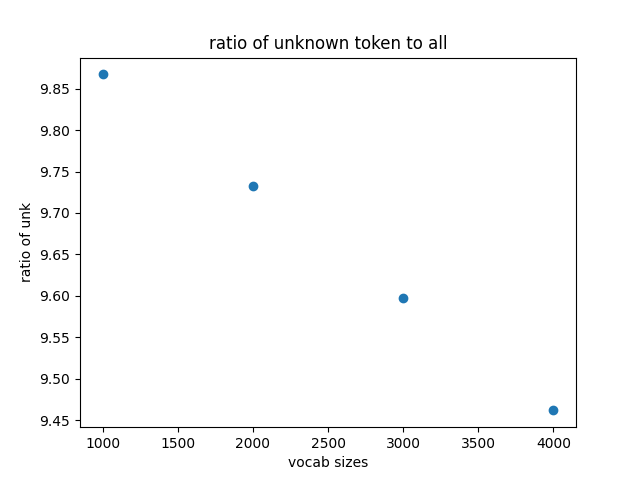
\includegraphics[width=0.6\linewidth]{../../stats/tokenization/unk-percentage.png}
        \caption{UNK token ratio}
    \end{center}
\end{figure}

\section{Language Model}
\subsection{Implementation Approach}
This section tries to fine tune our dataset on \textit{"GPT2-Medium"} and after fine tuning models will be saved. The saved model is then used to
generate a text on each labels. \\
At first I was continuing with default \textit{GPT2-Medium} but it didn't created a meaningful sentence then I tried to use some persian model that I came up with \href{https://huggingface.co/flax-community/gpt2-medium-persian}{GPT2-Persian} that would result in much better generation.
models are saved into \textit{models/[IE].language\_model}.I will just cover the first trait \textit{I,E} with more details.

\subsection{Results}
The examples of each labels are generated and then saved under the \textit{stats/language\_model} folder. So you can check their meaningfulness. I will get through the
\textit{I\_example.txt} and \textit{E\_example.txt}. As we know recgonzing personality detection is such a hard task for even psychologist. for example with one or five sentences
nobody can tell whether this person is Intorvert or Extrovert. But as much as I can, I'll check the generated sentences. we know that Extrovert people are more sociable and they tend to more
interact with other people on the other hand Introvert people tend to be more isolated and don't like to communicate with other people and they are shy person.
\begin{figure}[H]
    \begin{center}
        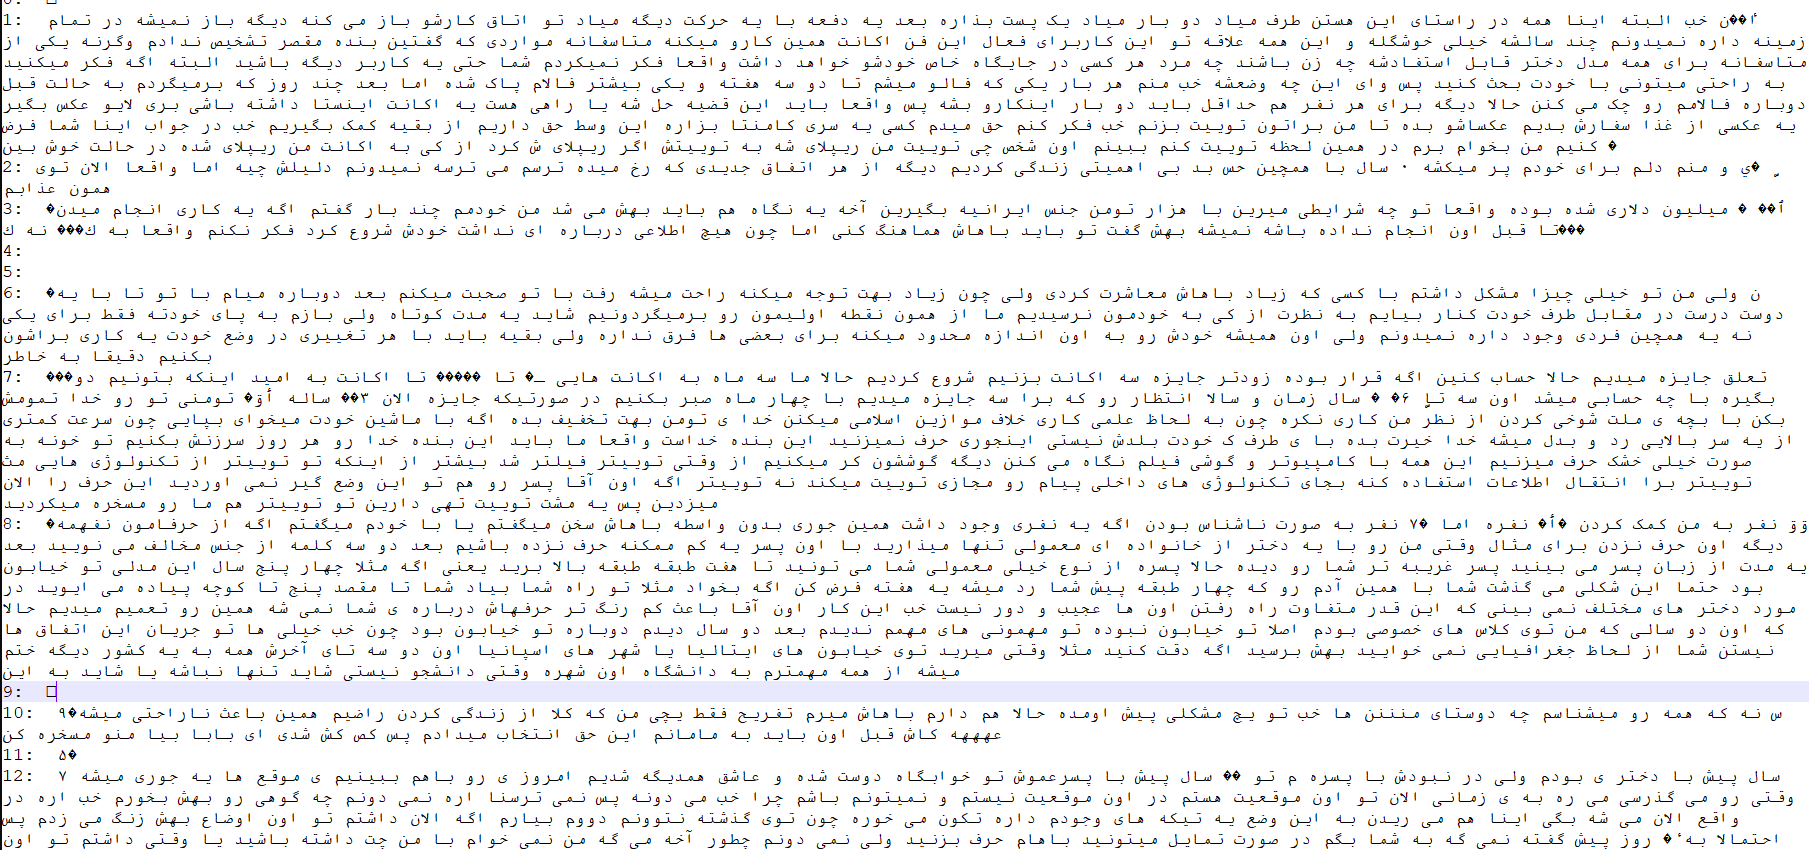
\includegraphics[width=1\linewidth]{../../stats/language_model/E_example.png}
        \caption{E example generated}
    \end{center}
\end{figure}
\begin{figure}[H]
    \begin{center}
        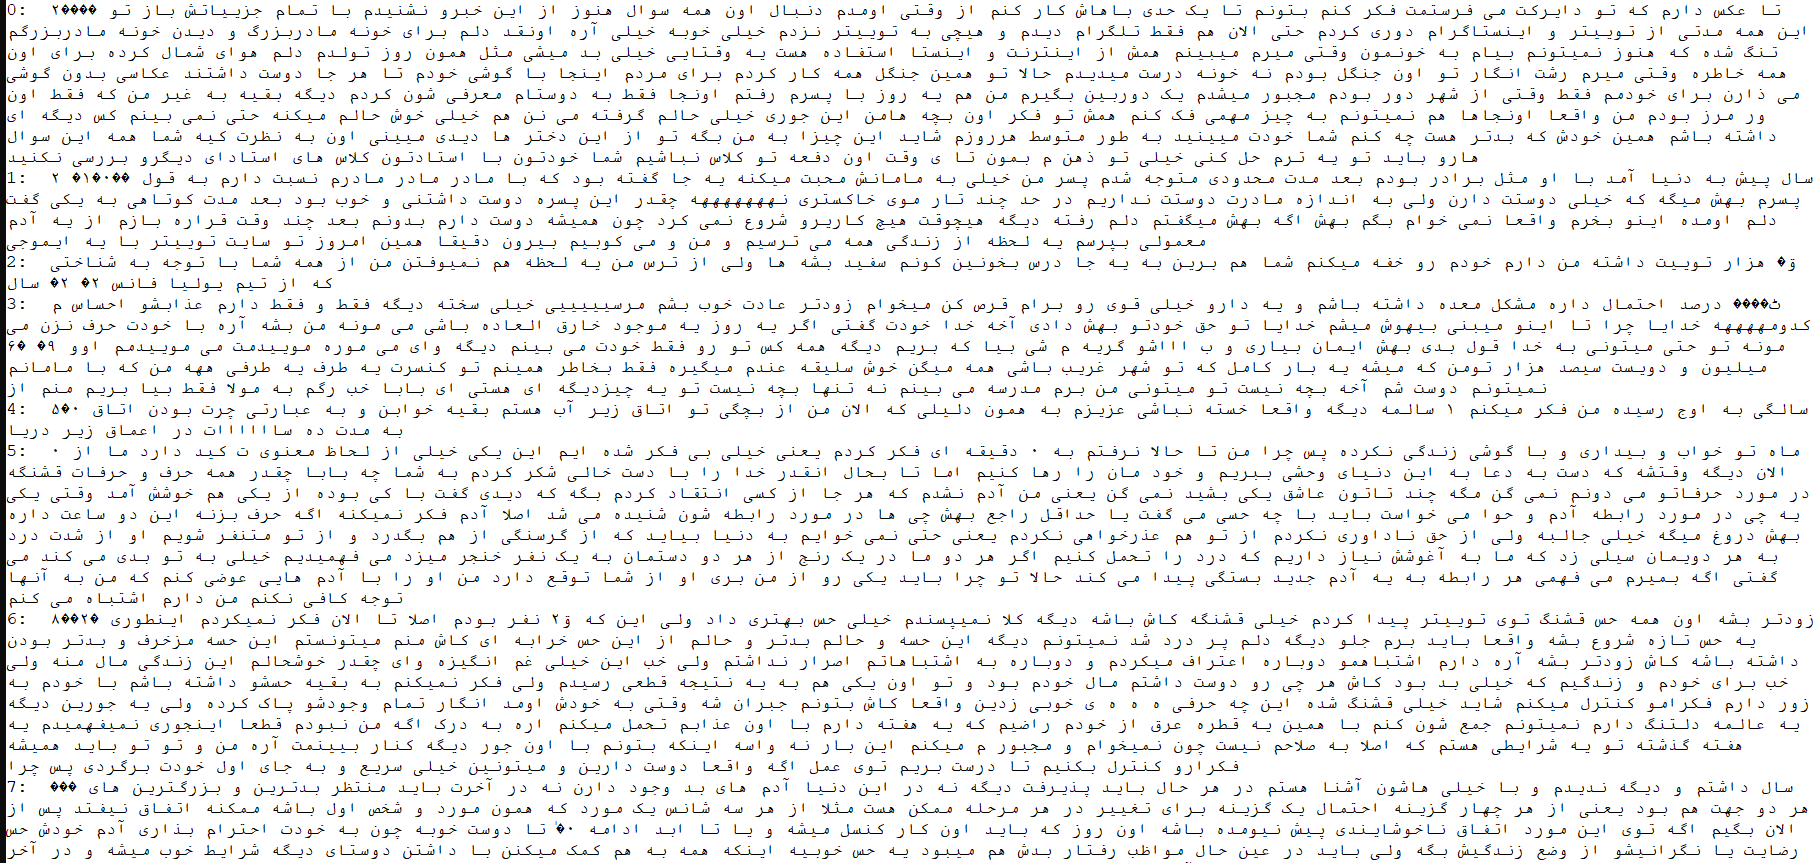
\includegraphics[width=1\linewidth]{../../stats/language_model/I_example.png}
        \caption{I example generated}
    \end{center}
\end{figure}

let's take a closer look at what "Introvert" person have said in first sentence : \fa{"این همه مدتی از توییتر و اینستاگرام دوری کردم حتی الان هم فقط تلگرام دیدم و هیچی به توییتر نزدم خیلی خوبه خیلی آره اونقد دلم برای خونه مادربزرگ و دیدن خونه مادربزرگم"}. As we
see this person tend to be more away from people and likes her past moments and don't want to socialize with other people.
But if we examine a 8th sentence of "Extrovert" person : \fa{"اگه یه نفری وجود داشت همین جوری بدون واسطه باهاش سخن میگفتم"}. so this behavior is only seen in Extrovert
people because they like to talk and they have capability to talk to other people even if they dont know them.

\section{Feature Engineering}
\subsection{Implementation Approach}
In this part our aim was to compare diffenret features and to conclude if we feed other feature besies our text data to our model, would model generalize and make decision better or not?
\\
So I defined a Neural Network model which can accept all of the features that I mention in next part. my model features was:
\begin{itemize}
    \item model architecture :
          \begin{itemize}
              \item a input size of 768 nuerons(for sake of generalizing like BERT).
              \item hidden layer of size 1000 with relu activation and dropout layer.
              \item hidden layer of size 200 with relu activation and dropout layer.
              \item output layer with one neuron and sigmoid activation
          \end{itemize}
    \item model settings:
          \begin{itemize}
              \item loss : Binary Cross Entropy
              \item optimizer : Adam with learning rate = 0.001
              \item epochs : 60
              \item batch size : 32
          \end{itemize}
\end{itemize}
inputs were fed in \textit{"cuda"} format for utilization from gpu and training faster.
\\
the features used in this experiments are exaplained below and I will get through the details of each input to be feedable to our model:
\begin{itemize}
    \item sentence length : an array that first number in array is sentence length and the array was padded with zero to be in length 768.
    \item word length : an array that fills word length through 768 elements of it. if tweets has more word than 768 it will be truncated and if tweets has less length than 768 will be padded with zero to be in length 768
    \item words : assigning unique number to each word. I first created a \textit{token dict} that each word has its unique number. And then tweets are tokenized each tokenized word are then mapped to their indexes. matching the dimension criterion was applied like previous approach.
    \item words-bigrams : just like previous feature but every consecutive two tokens are concatenated to represent one element of our array. array was filled until to get length 768. otherwise it will be padded by zero.
    \item word2vec : trained \textit{all.word2vec.npy} model were used to extract each token vectors from it. and then vectors extracted are summed to be in same direction and then it was fed into model.
    \item word2vec-bigram : treated like before but for each two consecutive word two vectors are concatenated and then all these vectors are summed.
    \item ParsBERT : used \href{https://huggingface.co/HooshvareLab/bert-fa-base-uncased}{bert-fa-base-uncased} model to tokenize and then feed each tokenized input to extract vectors. like word2vec all these token vectors are summed to be in same dimension as model input.
\end{itemize}
models are saved into \textit{models/feat\_engineering\_\{feature\_name\}.pth}.
\subsection{Results}
since the whole plot wouldn't be located in one figure it has been plotted in multi figure.
\subsubsection{loss}
\begin{figure}[H]
    \centering
    \subcaptionbox{loss A}{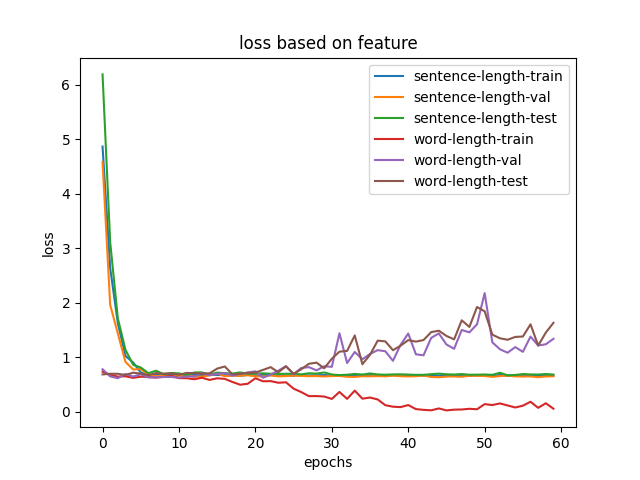
\includegraphics[width=0.33\textwidth]{../../stats/feat_engineering/loss/loss_feat_engineering_1.png}}%
    \hfill % <-- Seperation
    \subcaptionbox{loss B}{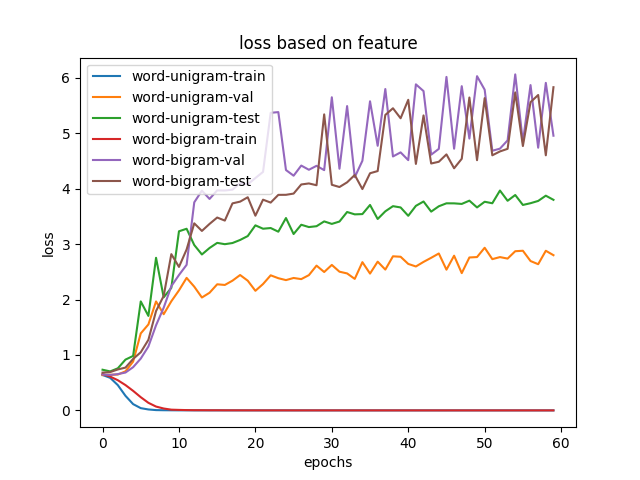
\includegraphics[width=0.33\textwidth]{../../stats/feat_engineering/loss/loss_feat_engineering_2.png}}%
    \hfill
    \subcaptionbox{loss C}{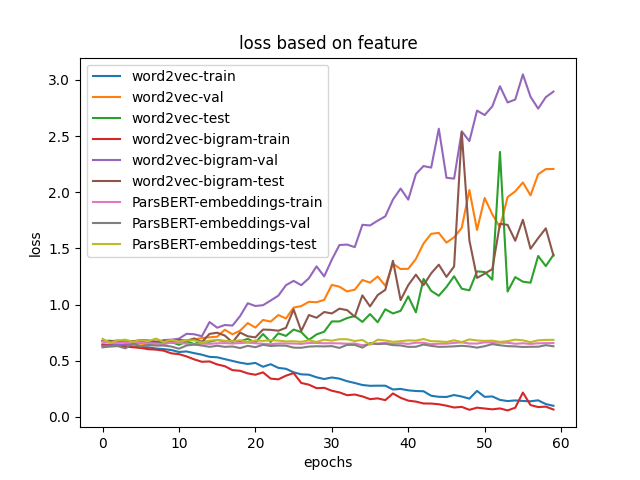
\includegraphics[width=0.33\textwidth]{../../stats/feat_engineering/loss/loss_feat_engineering_3.png}}%
    \caption{loss over 7 trained model on 3 parts train / val / test}
\end{figure}
Figure 1 : As we see sentence length model on each 3 parts have been covnerged well. but word length model just perform fantastic in train part but on test and val doesn't generalize well.
so it shows there is over-fit word length model. \\
Figure 2 : former behaviour is also seen in word-unigram and word-bigram model, so these models also overfit to just train data.
\\
Figure 3 : both word2vec unigram and bi-gram are overfit to train data and they perform well on training data. best model seen so far can be ParsBERT model with a low loss and without any effect of overfitting.

\subsubsection{accuracy}
\begin{figure}[H]
    \centering
    \subcaptionbox{acc A}{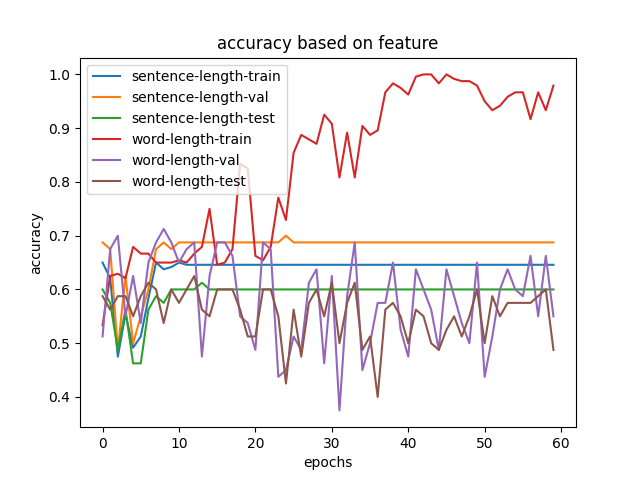
\includegraphics[width=0.33\textwidth]{../../stats/feat_engineering/acc/acc_feat_engineering_1.png}}%
    \hfill % <-- Seperation
    \subcaptionbox{acc B}{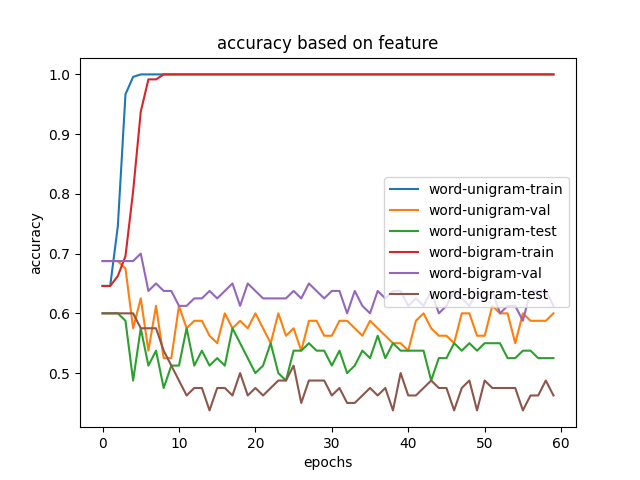
\includegraphics[width=0.33\textwidth]{../../stats/feat_engineering/acc/acc_feat_engineering_2.png}}%
    \hfill
    \subcaptionbox{acc C}{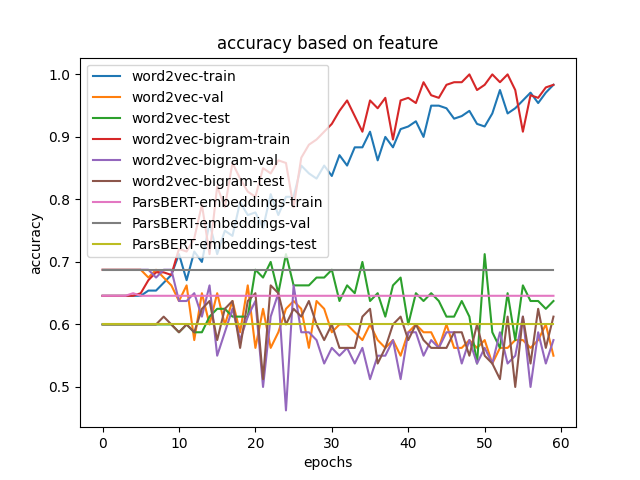
\includegraphics[width=0.33\textwidth]{../../stats/feat_engineering/acc/acc_feat_engineering_3.png}}%
    \caption{accuracy over 7 trained model on 3 parts train / val / test}
\end{figure}

If we look at three figures closely we'll see effect of overfitting on 5 models from our 7 models. the only two models that don't overfit are "sentence length" and "ParsBERT"
that ParsBERT with higher accuracy will defeat sentence length.

\section{Model Architecture}
\subsection{Implementation Approach}
As I see the progress on \textit{transformer} models in recent years. I chose my three models have some usage of transformer in it. I will dig through the 3 model architecture I have implemented.
\subsubsection{Word2Vec + ParsBERT}
This model involve both Word2Vec and ParsBERT together. such that my base model is Neural Netwerk and the logics are just like as I explained in prevoius section but the input I fed into this model
was vector of tokenized word on each model and then get average of these two different vecotrs and then feed it to the model. Since this model don't generlaize well(lack of sequence knowledge) I didnt try this model for other 3 traits.
\\
Model is save into models are saved into \textit{model\_architecture\_combined\_parsbert\_word2vec.pth} and the results of the models are convincing:
\begin{figure}[H]
    \centering
    \subcaptionbox{loss}{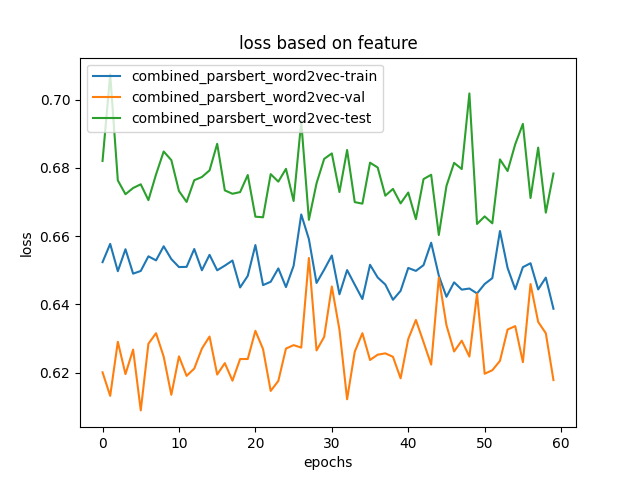
\includegraphics[width=0.49\textwidth]{../../stats/model_architecture/combined_ParsBert_word2vec/loss_model_architecture.png}}%
    \hfill % <-- Seperation
    \subcaptionbox{acc}{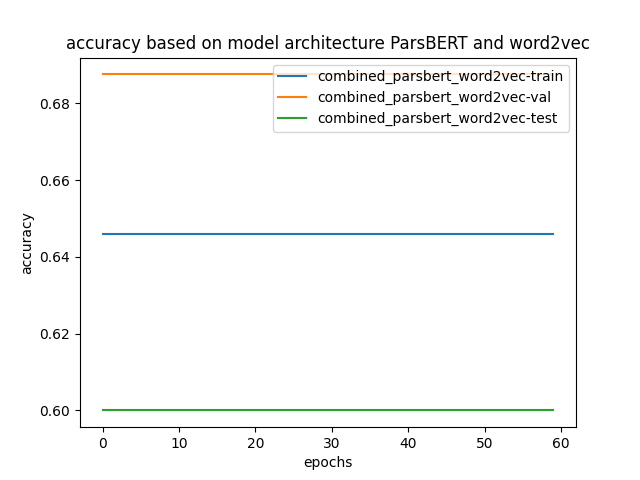
\includegraphics[width=0.49\textwidth]{../../stats/model_architecture/combined_ParsBert_word2vec/acc_model_architecture.png}}%
    \caption{accuracy over 7 trained model on 3 parts train / val / test}
\end{figure}

\subsubsection{BERT Truncated}
As in the name of section says, this model are feed tweets with truncated length to be not more than 512 tokens. during training this model, I have ran into serious GPU out of memory issue and
I have tried many different solutions to overcome this problem. for example I used the built in \textit{Trainer} object of pytroch for training or I decreased length of sentence which didn't lead
to be escape way. At the end I tried to lowered \textit{batch size} so that trade-off between batch size and model preserves. because lower batch size results in much more training time and higher
batch size will result in GPU shortage. So I chose \textit{batch size = 14} that happens to be the best batch size. through this batch size GPU usage was about 14GB. According to \textit{colab} free
account users don't have more than 15GB GPU.
\\

\textbf{Model Explaination}
\begin{enumerate}
    \item first of all I concatenated all tweets of user with space and this makes our input to be in string format instead of list.
    \item after that I make 4 individual trait for training 4 four different models. I meant that "I,E" are together and then binary classified, "S, N" are together and then binary classified and etc.
    \item then I splitted my dataset into 3 parts train/validation/test.
    \item I defined Custom model which uses BERT \text{CLS} embeddings which stands for classification. and with this embeddings I managed to build a fully connected layer which maps (768, 1). as we
          know our output neuron should be one because we have binary classification and use sigmoid as activation function. and \textit{BCELoss} for loss function and AdamW for optimizer. And in the end model was trained on 8 epochs.
    \item I make use of pretrained \href{https://huggingface.co/HooshvareLab/bert-fa-base-uncased}{ParsBERT model} as my pretrained BERT embeddings.
    \item Fine-tuning phase is applied on all layer even BERT layer.
    \item The model is saved into \textit{models/BERT\_TRUNCATED\_MODEL}
\end{enumerate}

let's take a look at models resutls:
\begin{figure}[H]
    \centering
    \subcaptionbox{I/E traits}{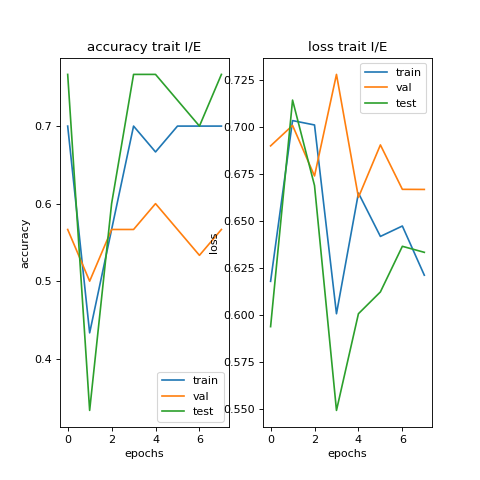
\includegraphics[width=0.49\textwidth]{../../stats/model_architecture/bert_truncated/trait_0.png}}%
    \hfill % <-- Seperation
    \subcaptionbox{S/N traits}{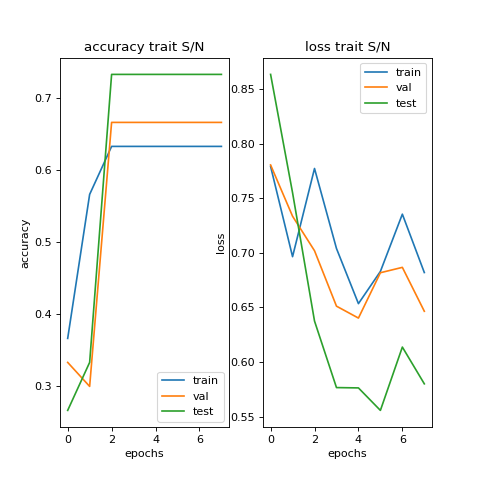
\includegraphics[width=0.49\textwidth]{../../stats/model_architecture/bert_truncated/trait_1.png}}%
\end{figure}
\begin{figure}[H]
    \centering
    \subcaptionbox{T/F traits}{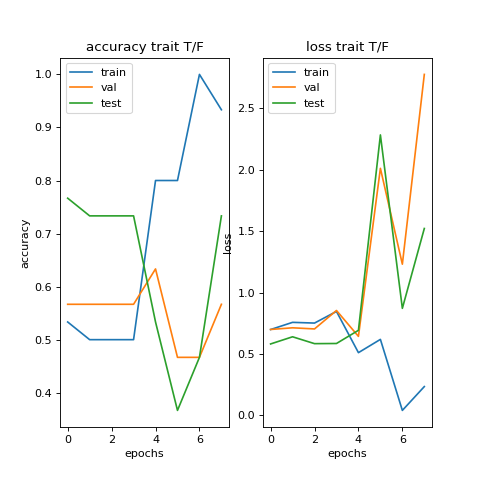
\includegraphics[width=0.49\textwidth]{../../stats/model_architecture/bert_truncated/trait_2.png}}%
    \hfill % <-- Seperation
    \subcaptionbox{P/J traits}{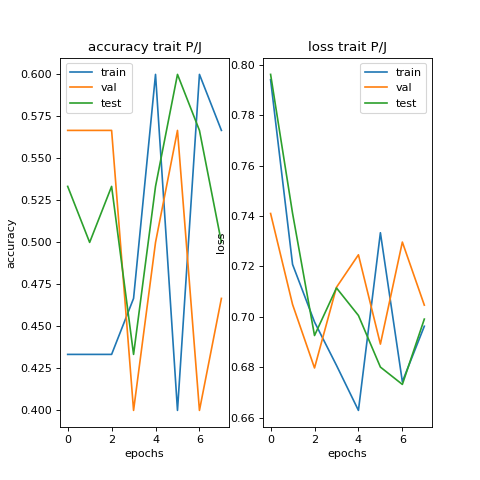
\includegraphics[width=0.49\textwidth]{../../stats/model_architecture/bert_truncated/trait_3.png}}%
\end{figure}

As we see in all of 4 traits test data has acheived acceptable accuracy and its more than 70 percentage in all of them. that means we have made a progress in that way. and we don't see any overfit or at least a little overfit on our data which is great.

\subsubsection{BERT Into BERT}
This my final model which after consulting with many senior in NLP field and my mentors I came up into it. In fact I have about 4000 users and collected all of their tweets which on average each user has 700 tweets.
And if we count each tweet has at least 30 tokens, for each user I have 21000 tokens and for a model like bert which at most can be feed 512 tokens it's such a enormous challenge.
\begin{enumerate}
    \item So the idea was to leverage each user as a batch(that cleary make our batch size length = 1).
    \item and then feed all tweets into a embedding bert that would result in shape \textit{(tweets\_length, sequence\_length, dimension)}
    \item then we extract CLS embedding to have shape \textit{(tweets\_length, dimension)}
    \item so in this step we have repsresenation for each tweet(embedding for each tweet)
    \item now we feed the extracted CLS embeddings to another bert
    \item on top of the second BERT we extracted CLS layer and then feed it into a fully connected layer for binary classification.
    \item At first I tried to fine-tune on 2 BERTs but because lack of GPU memory I had to just fine-tune on the second BERT. Altough fine-tuning on second BERT is a great approach.
\end{enumerate}
the model is saved under \textit{models/bert\_in\_bert} directory.
\newpage
let's take a look at the model results:
\begin{center}
    \begin{adjustbox}{max width=0.8\textwidth}
        \csvautotabular{../../stats/model_architecture/bert_into_bert/outputs_bert_into_bert_0.csv}
    \end{adjustbox}
    % \vspace*{1cm}
\end{center}
\begin{center}
    I/E trait
\end{center}
\begin{center}
    \begin{adjustbox}{max width=0.8\textwidth}
        \csvautotabular{../../stats/model_architecture/bert_into_bert/outputs_bert_into_bert_1.csv}
    \end{adjustbox}
\end{center}
\begin{center}
    S/N trait
\end{center}

\begin{center}
    \begin{adjustbox}{max width=0.8\textwidth}
        \csvautotabular{../../stats/model_architecture/bert_into_bert/outputs_bert_into_bert_2.csv}
    \end{adjustbox}
\end{center}
\begin{center}
    T/F trait
\end{center}

\begin{center}
    \begin{adjustbox}{max width=0.8\textwidth}
        \csvautotabular{../../stats/model_architecture/bert_into_bert/outputs_bert_into_bert_3.csv}
    \end{adjustbox}
\end{center}
\begin{center}
    P/J trait
\end{center}
as we see \textit{test} part on first 3 trait are above 70 percentage that is great but for the 4th trait model hasn't performed well.
\\
\textbf{So all in all the \textit{"BERT Into BERT"} model outperforms other models and it's picked as our idol model.}

\section{Data Augmentation}
\subsection{Implementation Approach}
At first I got ChatGPT api key. and then I make truncated text from list of tweets since tweets length exceeds ChatGPT api free access.
then I fine tuned chatgpt on my data(chosen model was \textit{text-davinci-003}). After fine tuning I iterated over 16 possible labels and inside this labels I've randomly chosen some rows.
within selected row I concatenated each tweets into string and I made a prompt like this:
\\
\textit{"I want you to act as a Data Augmenter Specialist. I will provide you some users tweets and their related MBTI types.
    And then I want you to make a tweet that a person with that MBTI type would tweet. tweets examples are provided below:
    \{tweets : \textit{some sample tweets concatenated 1}, mbti\_type:\textit{some label from 16 labels 1}\},\{tweets : \textit{some sample tweets concatenated 2}, mbti\_type:\textit{some label from 16 labels 2}\}"}

\subsection{Results}
\begin{figure}[H]
    \begin{center}
        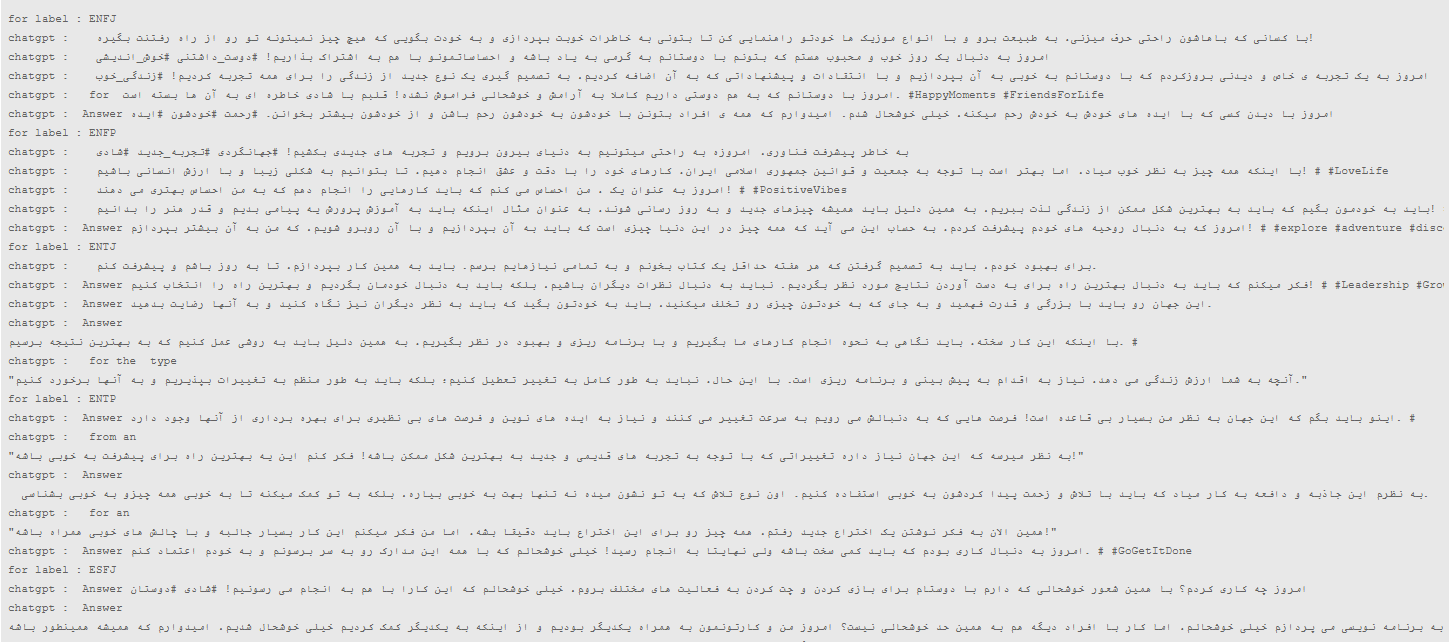
\includegraphics[width=1\linewidth]{./images/data-aug.png}
        \caption{data generated for each trait by chatgpt}
    \end{center}
\end{figure}

\begin{figure}[H]
    \begin{center}
        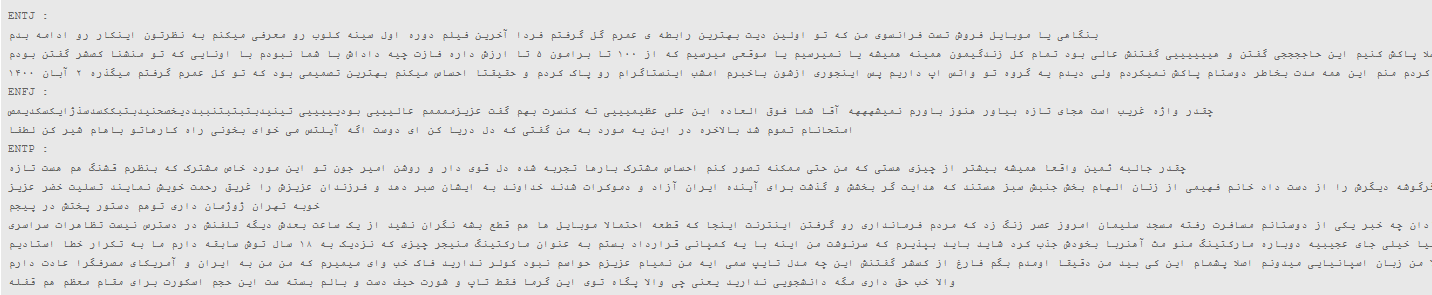
\includegraphics[width=1\linewidth]{./images/actual-data.png}
        \caption{actual data in our dataset}
    \end{center}
\end{figure}
As we see there is high resemblance in data created by GPT and our actual data. but GPT in someway lost the context in between its sentence
but it can ends its sentence much well.

\section{Zero Shot Classification by GPT}
\subsection{Implementation Approach}
As I said earlier because GPT max token is 4097 and my tokens is much greater than this number I had to truncate my tweet until it can be requested to GPT.
like previous part my chosen model was \textit{text-davinci-003}. after that I fed the truncated tweets to model and asked model to generate their label from 16 possible labels.
my prompt was in this format:
\\
\textit{"You are picking the labels for a zero shot classification model on user tweets, domain is MBTI personality types, Generate a label from 16 MBTI types. tweet is : `\{some tweet from user\}`"}
\\
Unfortunately I encountered \textit{RateLimitError} request that I couldn't accomplish this task.
% \subsection{Result}

\end{document}


